\newpage

\chapter{Experimental Setup}

The whole experimental system consisted of a QT generator and two second sound sensors, which were placed into a cylindrical resonator cavity of diameter $ d=10\unit{mm}$ and height $ H=65\unit{mm} $. One of the second sound sensors (speaker) is connected to the waveform generator and the other one (receiver) to a SR-830 lock-in amplifier. A more detailed description is presented later in this chapter.


\section{Quantum Turbulence Generator}

Quantum turbulence can be produced by any oscillating objects such as grids, tuning forks or spheres. In our experiment we used an oscillating piezoelectric tuning fork, fully controlled electrically. 

\subsection*{Quartz Tuning Fork}

In general, quartz tuning forks are commercially produced piezoelectric oscillators. Their most common application is as frequency standards in digital watches or other electronic components.
We used a custom-made fork with fundamental resonance at $ f_0 = 6500\unit{Hz} $ in vacuum at room temperature. The geometry of the fork is sketched in {\sffamily\textbf{Figure 2.1}}.

\begin{wrapfigure}{r}{0.23\textwidth}
	\centering
	\vspace{-0.8cm}
	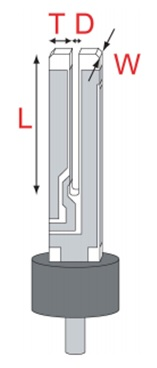
\includegraphics[width=0.20\textwidth]{graphics/quartz}
	\caption{Sketch of quartz tuning fork.}
	\vspace{-1.8cm}	
\end{wrapfigure}

The size of the fork is given by prong length $ \mathcal{L} = 3.5\unit{mm} $, prong width $ \mathcal{W}=75 \mu\text{m} $, thickness $ \mathcal{T}=90\mu\text{m} $ and the distance between prongs $ \mathcal{D}=90\mu\text{m} $. The fork was driven by an amplified alternating voltage $ U\propto e^{i\omega t} $, causing the anti-phase lateral oscillation of fork's prongs. The first flexural overtone can be found at the frequency $ f_1 = 40\unit{kHz} $. In this resonant mode, there are two nodes and anti-nodes along the length of the prongs (one anti-node is at the supporting base). In both cases there is an upper boundary for the amplitude of AC voltage. Exceeding this value will cause the prongs to hit each other repeatedly, which could result in serious damage.
\\
Two other important properties of fork are the effective mass of one prong $ m_{\text{eff}} $ and a so-called fork constant $ a $. For our case, we can estimate them (using formulas and data from\cite{forks, acoustic}) as:
\begin{align}
m_{\text{eff}}&=\frac{1}{4}\mathcal{L}\mathcal{T}\mathcal{W}\rho_q = 1.52 \cdot 10^{-8} \unit{kg}\,,\nonumber\\
a_{\text{fund}}&= 3.61 \cdot 10^{-7} \unit{Cm}^{-1}\,,\nonumber\\
a_{\text{over}}&= 1.38 \cdot 10^{-6} \unit{Cm}^{-1}\,,\nonumber
\end{align}
where $ \rho_q = 2650 \unit{kg/m}^3 $ is the quartz density. Values of the fork constants were taken from\cite{acoustic}, where tuning forks of the same parameters and from the same series were used.

It was also shown\cite{forks} that by applying AC voltage with amplitude $ U_{A} $ results in a driving force acting on the fork's prongs of magnitude $ F = \frac{1}{2}aU $. Moreover, by measuring the current response $ I $ we can determine the velocity at the tip of the prongs as $ v=I/a $. Knowledge of these parameters is crucial for all measurements related with superfluid hydrodynamics.

\section{Second Sound Source and Detector}

Second sound is a wave of temperature and entropy, but can be produced purely mechanically. In particular, when a semi-permeable membrane with sub-micron pores is oscillating in He-II, the superfluid component can flow through the pores much easier than the normal component (due to the lack of viscosity). Thus, its oscillation will push only the normal component and consequently, this creates (due to continuity equations) a local oscillation of densities $ \rho_{\ind n} $, $ \rho_{\ind s} $ and hence, a longitudinal wave of second sound. At the right frequency of oscillation, this results in a resonant second-sound standing wave in the experimental cylindrical cavity.

In our experiment we used two identical sensor devices to produce and also detect the second sound. The sensor itself is essentially a capacitor where one electrode consists of the membrane with a 100~nm thick gold layer above the surface and the other electrode is made of brass. The full sketch and photo can be seen in {\sffamily\textbf{Figure 2.2}}.

\begin{figure}[h]
	\centering
	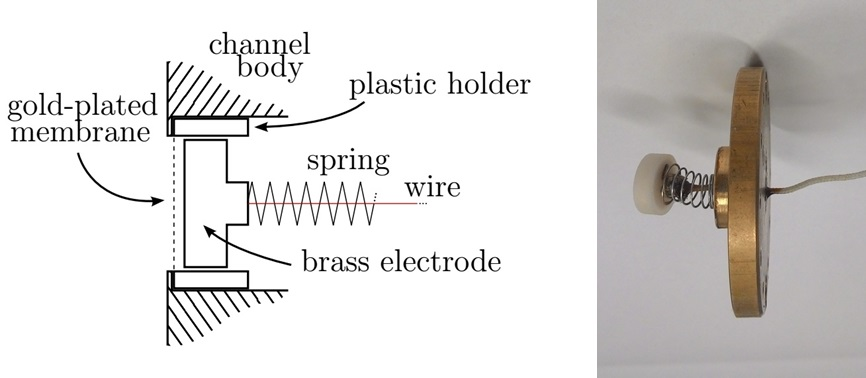
\includegraphics[width=0.7\textwidth]{graphics/SSpic}
	\caption{Left: Technical sketch showing the parts of the second sound sensor. Right: A photograph of our experimental construction.}
\end{figure}

The gold electrode is electrically connected with the resonator body while the other electrode to the wave generator or lock-in amplifier (depends whether the device is set as a speaker or receiver). Together, these electrodes form a capacitor of $\approx 60-100\unit{pF}$ and applying an AC voltage (units of Volts) superimposed on a 90~V DC bias causes the oscillation of the membrane and therefore production of second sound.

Because of finite distance between the sensors $ H $, we observe many harmonic resonance modes. The resonance frequency can be estimated from the equation for standing waves:

\begin{equation}
f = \frac{u_2}{\lambda} = \frac{u_2}{2H}n\,.
\label{SSresonance}
\end{equation}

\newpage

\section{The Apparatus}

We have introduced the principle of making quantum turbulence and also its detection. In this section we describe the necessary technical parts of the experiment in more detail.

\subsection*{Resonator}

As mentioned above, the quartz tuning fork and both second sound devices were placed into the cylindrical resonator cavity. The fork is located in the middle and the second sound sensors at each end of the resonator, facing each other. 

\begin{figure}[h]
	\centering
	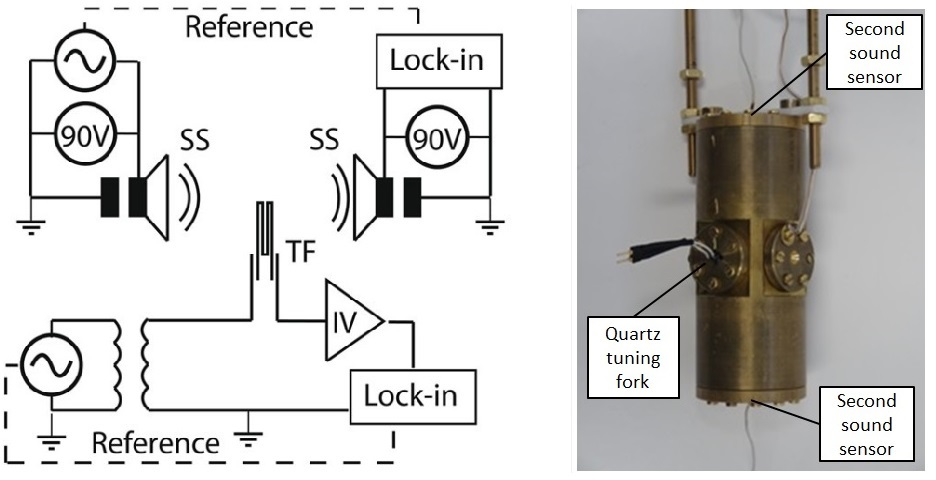
\includegraphics[width=0.7\textwidth]{graphics/setup}
	\caption{Left: Electrical schematics of the setup. Right: Photograph of the resonator.}
\end{figure}

A small 1~mm thin hole is drilled through the body, connecting the cavity to the open bath filled with superfluid helium.

\subsection*{Insert}

\begin{wrapfigure}{r}{0.53\textwidth}
	\centering
	\vspace{-0.5cm}
	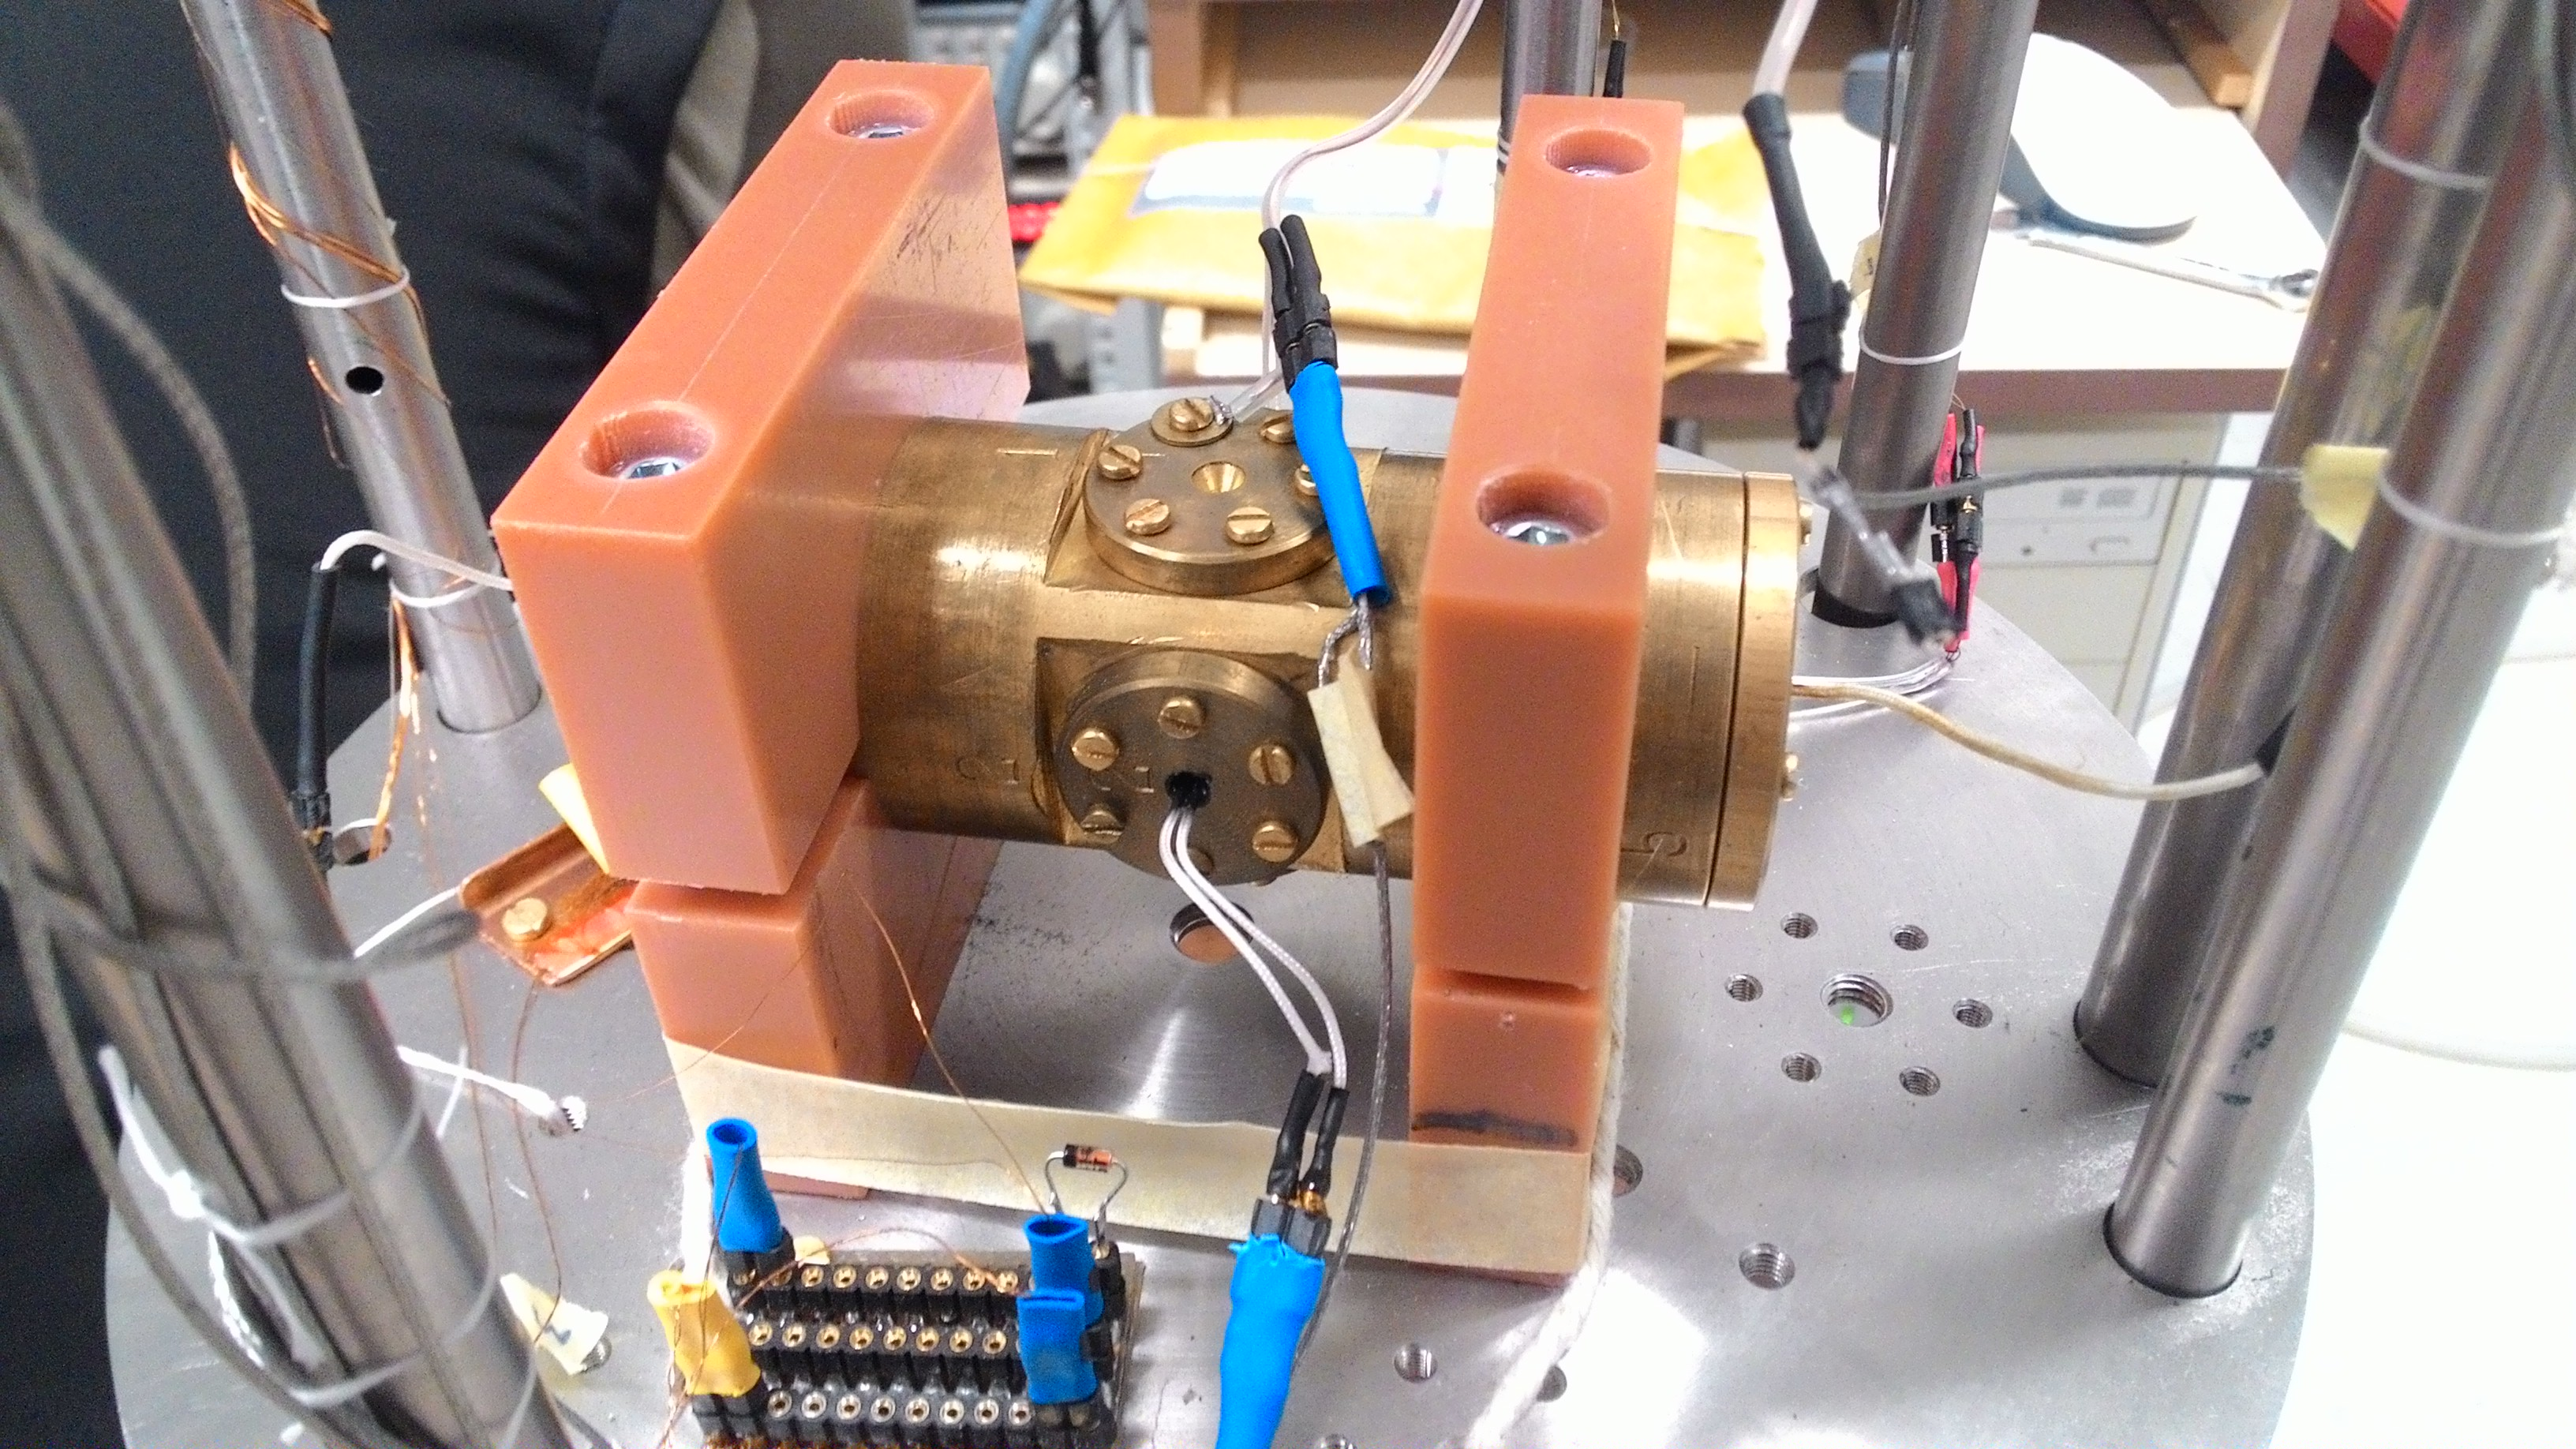
\includegraphics[width=0.5\textwidth]{graphics/photo_insert2}
	\caption{Photograph of the resonator fixed at the bottom of the insert.}
	\vspace{0cm}	
\end{wrapfigure}

To ensure a fixed location of the resonator inside the helium bath, we attached it at the bottom of the \textit{insert}. The cryogenic insert is a large metallic construction, to which all resistors, coaxial cables, and thermometers are attached. The total height of insert is comparable with the height of the cryostat, so when placed into a superfluid bath, the resonator will be located near the bottom. Since the helium level in cryostat is continuously decreasing, this location of resonator is optimal.


\subsection*{Cryostat}


The insert along with all important devices were put into a vessel, designed for working with cryogenic fluids. At the top, the cryostat allows access into the helium bath, but at the same time, the cryostat must be well-insulated from external heat fluxes.

After the cryostat was pre-cooled to liquid nitrogen (LN$_2$) temperature $ (\approx 77\unit{K}) $, we continued precooling with helium vapour and finally transferred liquid helium (LHe) at $ (\approx 4.2\unit{K}) $ from a transport dewar. Vapours from the rapidly evaporating LHe were immediately pumped by a set of Roots-pumps so that the inner pressure above the LHe surface was further decreased. Reducing the saturated vapour pressure provided the cooling even below $ T_{\lambda} $. This method works efficiently until the minimum temperature of $ \approx 1.25\unit{K} $ is reached.


\begin{figure}[h]
	\centering
	\vspace{0.5cm}
	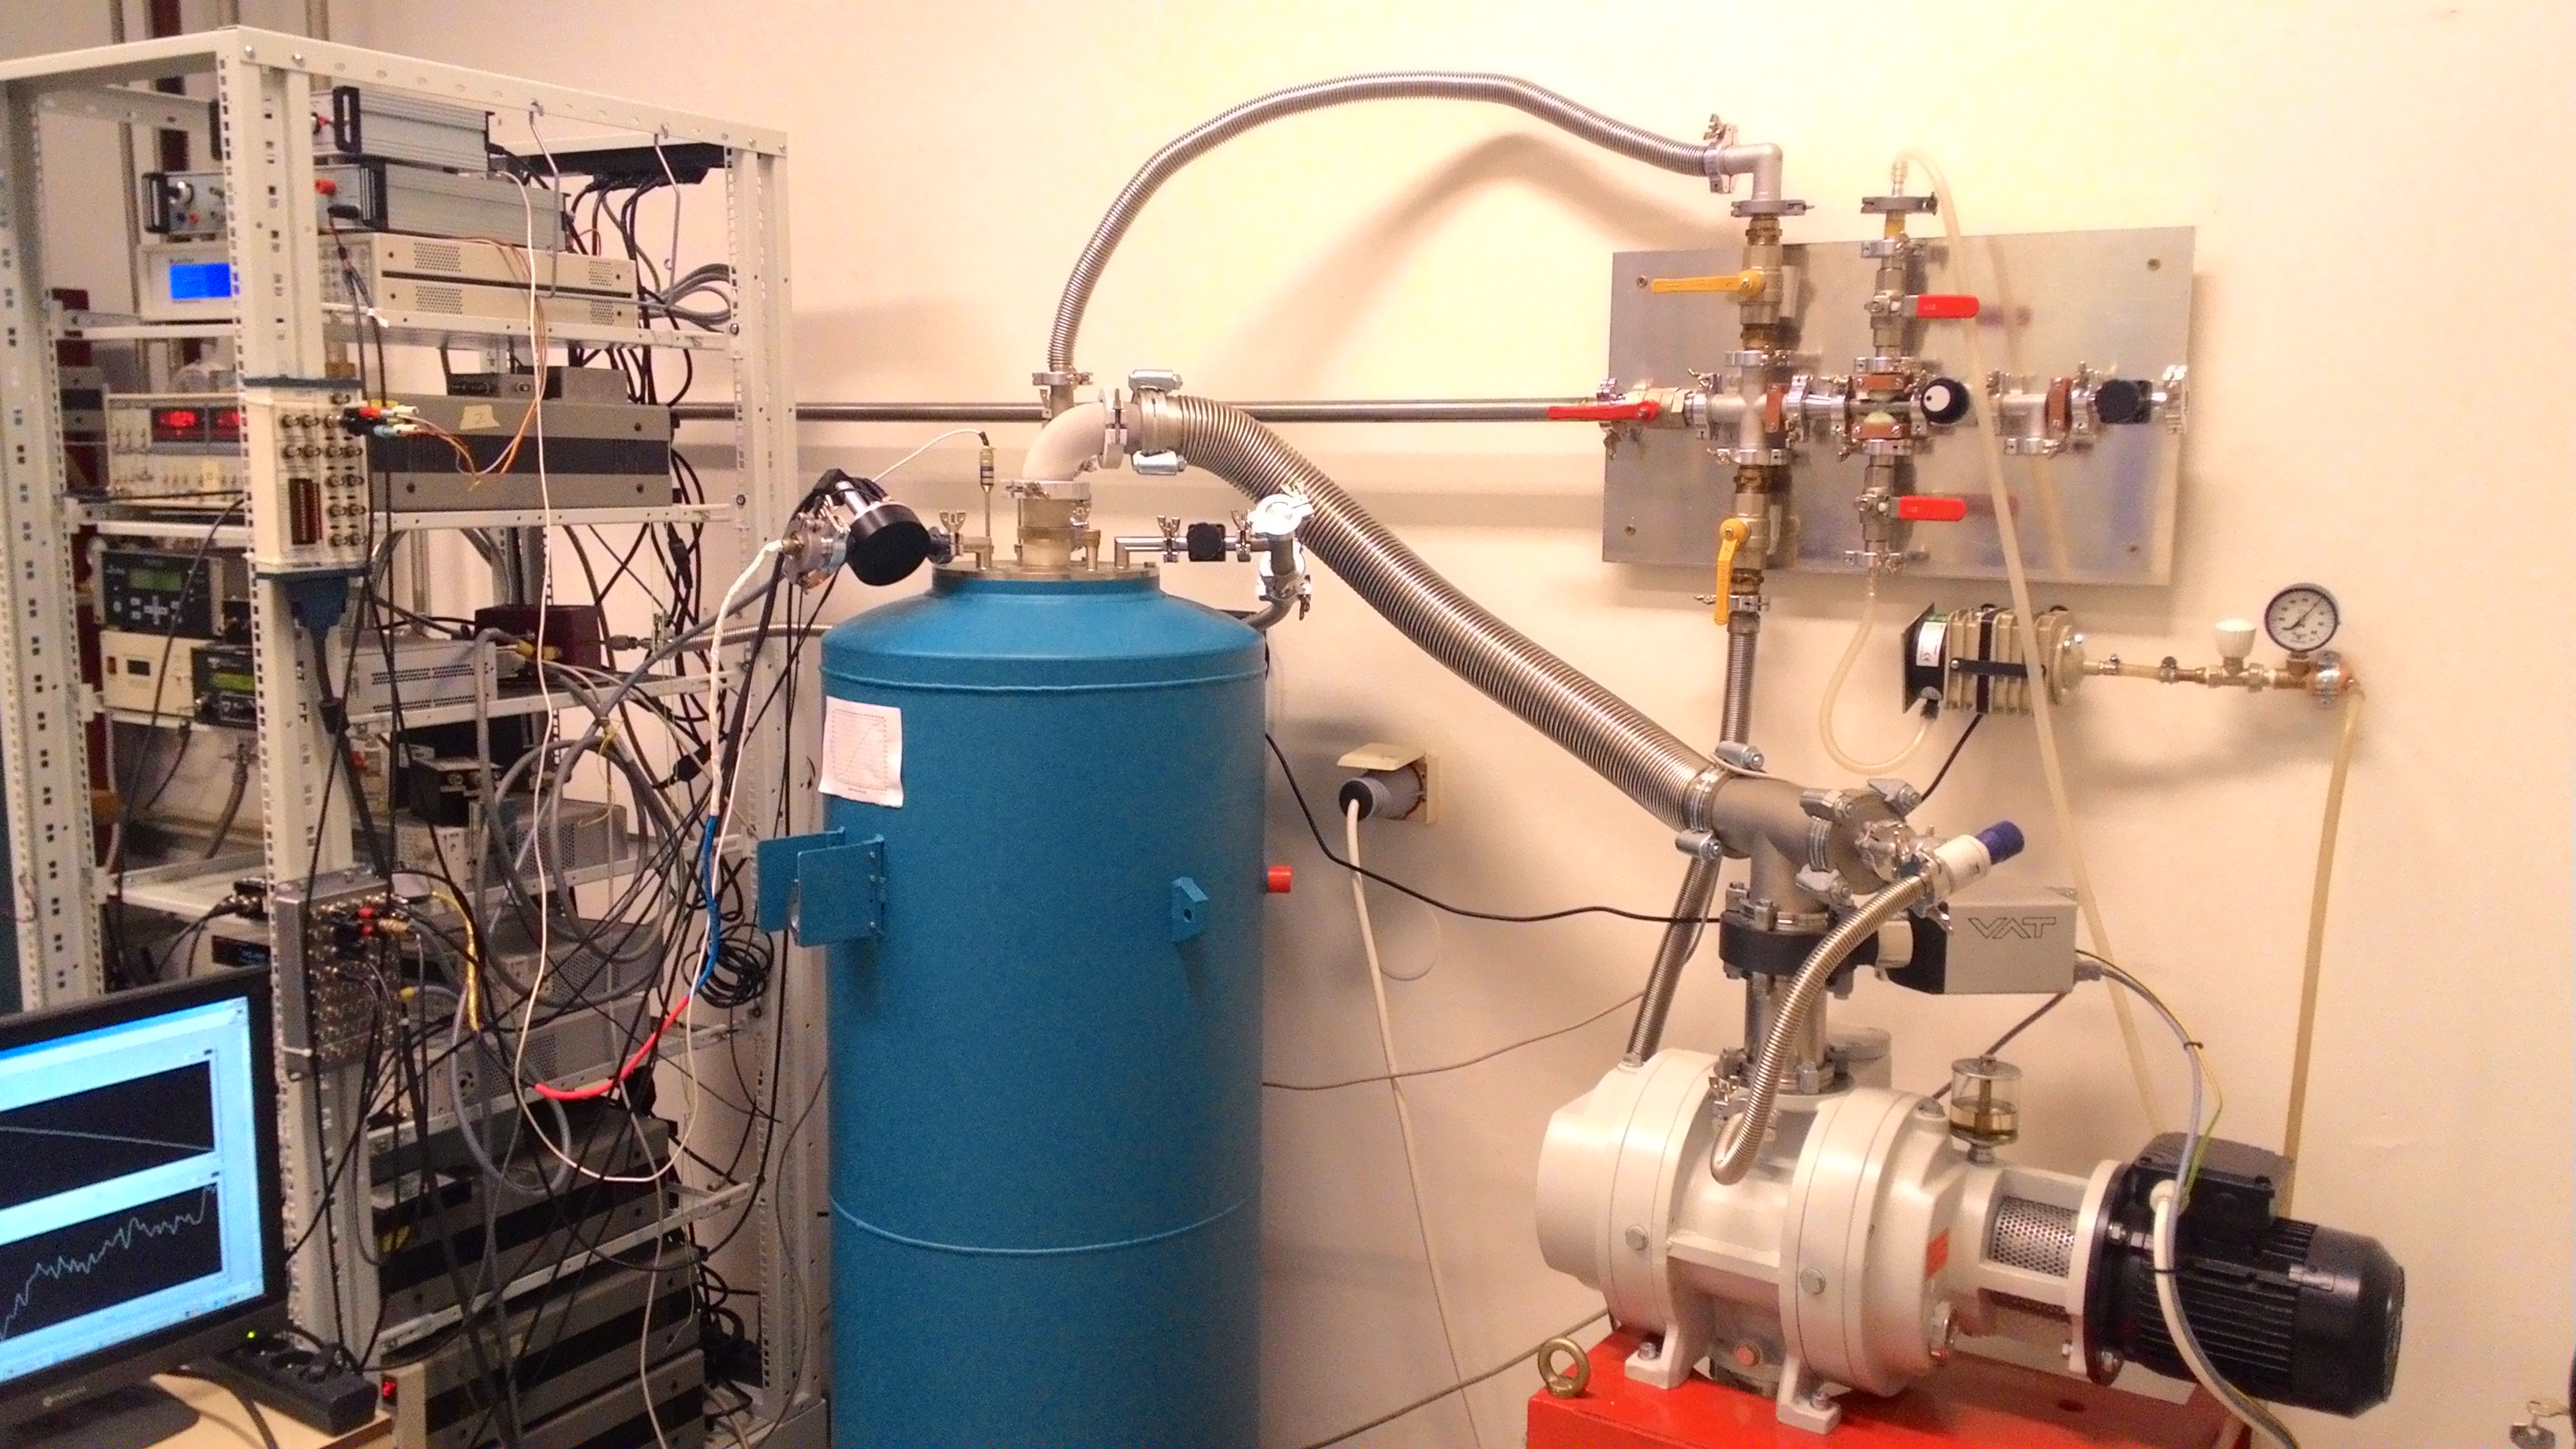
\includegraphics[width=0.8\textwidth]{graphics/apparatus}
	\caption{Photograph of the experimental setup - Left: waveform generators, lock-in amplifiers. Middle: cryostat, pipes where helium gas is flowing out of the system. Right: Roots-pump.}
\end{figure}

During the measurements it was crucial to have the temperature stabilized minimal deviations. Two methods have been used for measuring the temperature. The first was a direct resistance measurement of a miniature semiconductor thermometer (Germanium thin film on GaAs substrate) placed in the helium bath, with calibration known from previous experiments. The second method was a simple conversion between saturated vapour pressure and temperature based on \cite{donnelly}. The pressure was regulated (both manually and electronically) by manipulating the pump valve.

To summarize, we prepared a cooling system able to reach any temperature above $ \approx 1.25\unit{K} $. Overall, we did systematic measurements at 9 different temperatures: $ 2.15\unit{K} $, $ 2.05\unit{K} $, $ 2.00\unit{K} $, $ 1.95\unit{K} $, $ 1.80\unit{K} $, $ 1.65\unit{K} $, $ 1.60\unit{K} $, $ 1.55\unit{K} $, $ 1.35\unit{K}$. Although our total temperature range is less than $ 1\unit{K} $, there are dramatical changes in the composition of LHe. One can recall (graph in {\sffamily\textbf{Figure 1.3}}) that at $ 2.15\unit{K} $ there is only about $ 5\% $ of the superfluid component and at $ 1.35 \unit{K} $ it is more than $ 90\% $.


\newpage
\section{Measurement Methods}

Since we decided to focus on various aspects of the studied problem, we used several methods of measurement with the quartz tuning fork and second sound sensors, discussed in the following text.

\subsection*{Frequency Sweeps of the Tuning Fork}

In this mode the tuning fork was oscillating with a frequency that was changing along some chosen range. This was important for characterizing the fork resonance with its frequency $ f_0 $, width $ \Delta f $, signal amplitude $ U_0 $ and background signal (offset) $ U_{\text{off}} $. Frequency sweeps were made around the fundamental and overtone resonance frequencies $ f_0^{\ind f} = 6.38\unit{kHz} $, $ f_0^{\ind o} = 40.00\unit{kHz} $. Two examples of these measurements are shown in {\sffamily\textbf{Figure 2.6}}.

\begin{figure}[h]
	\centering
	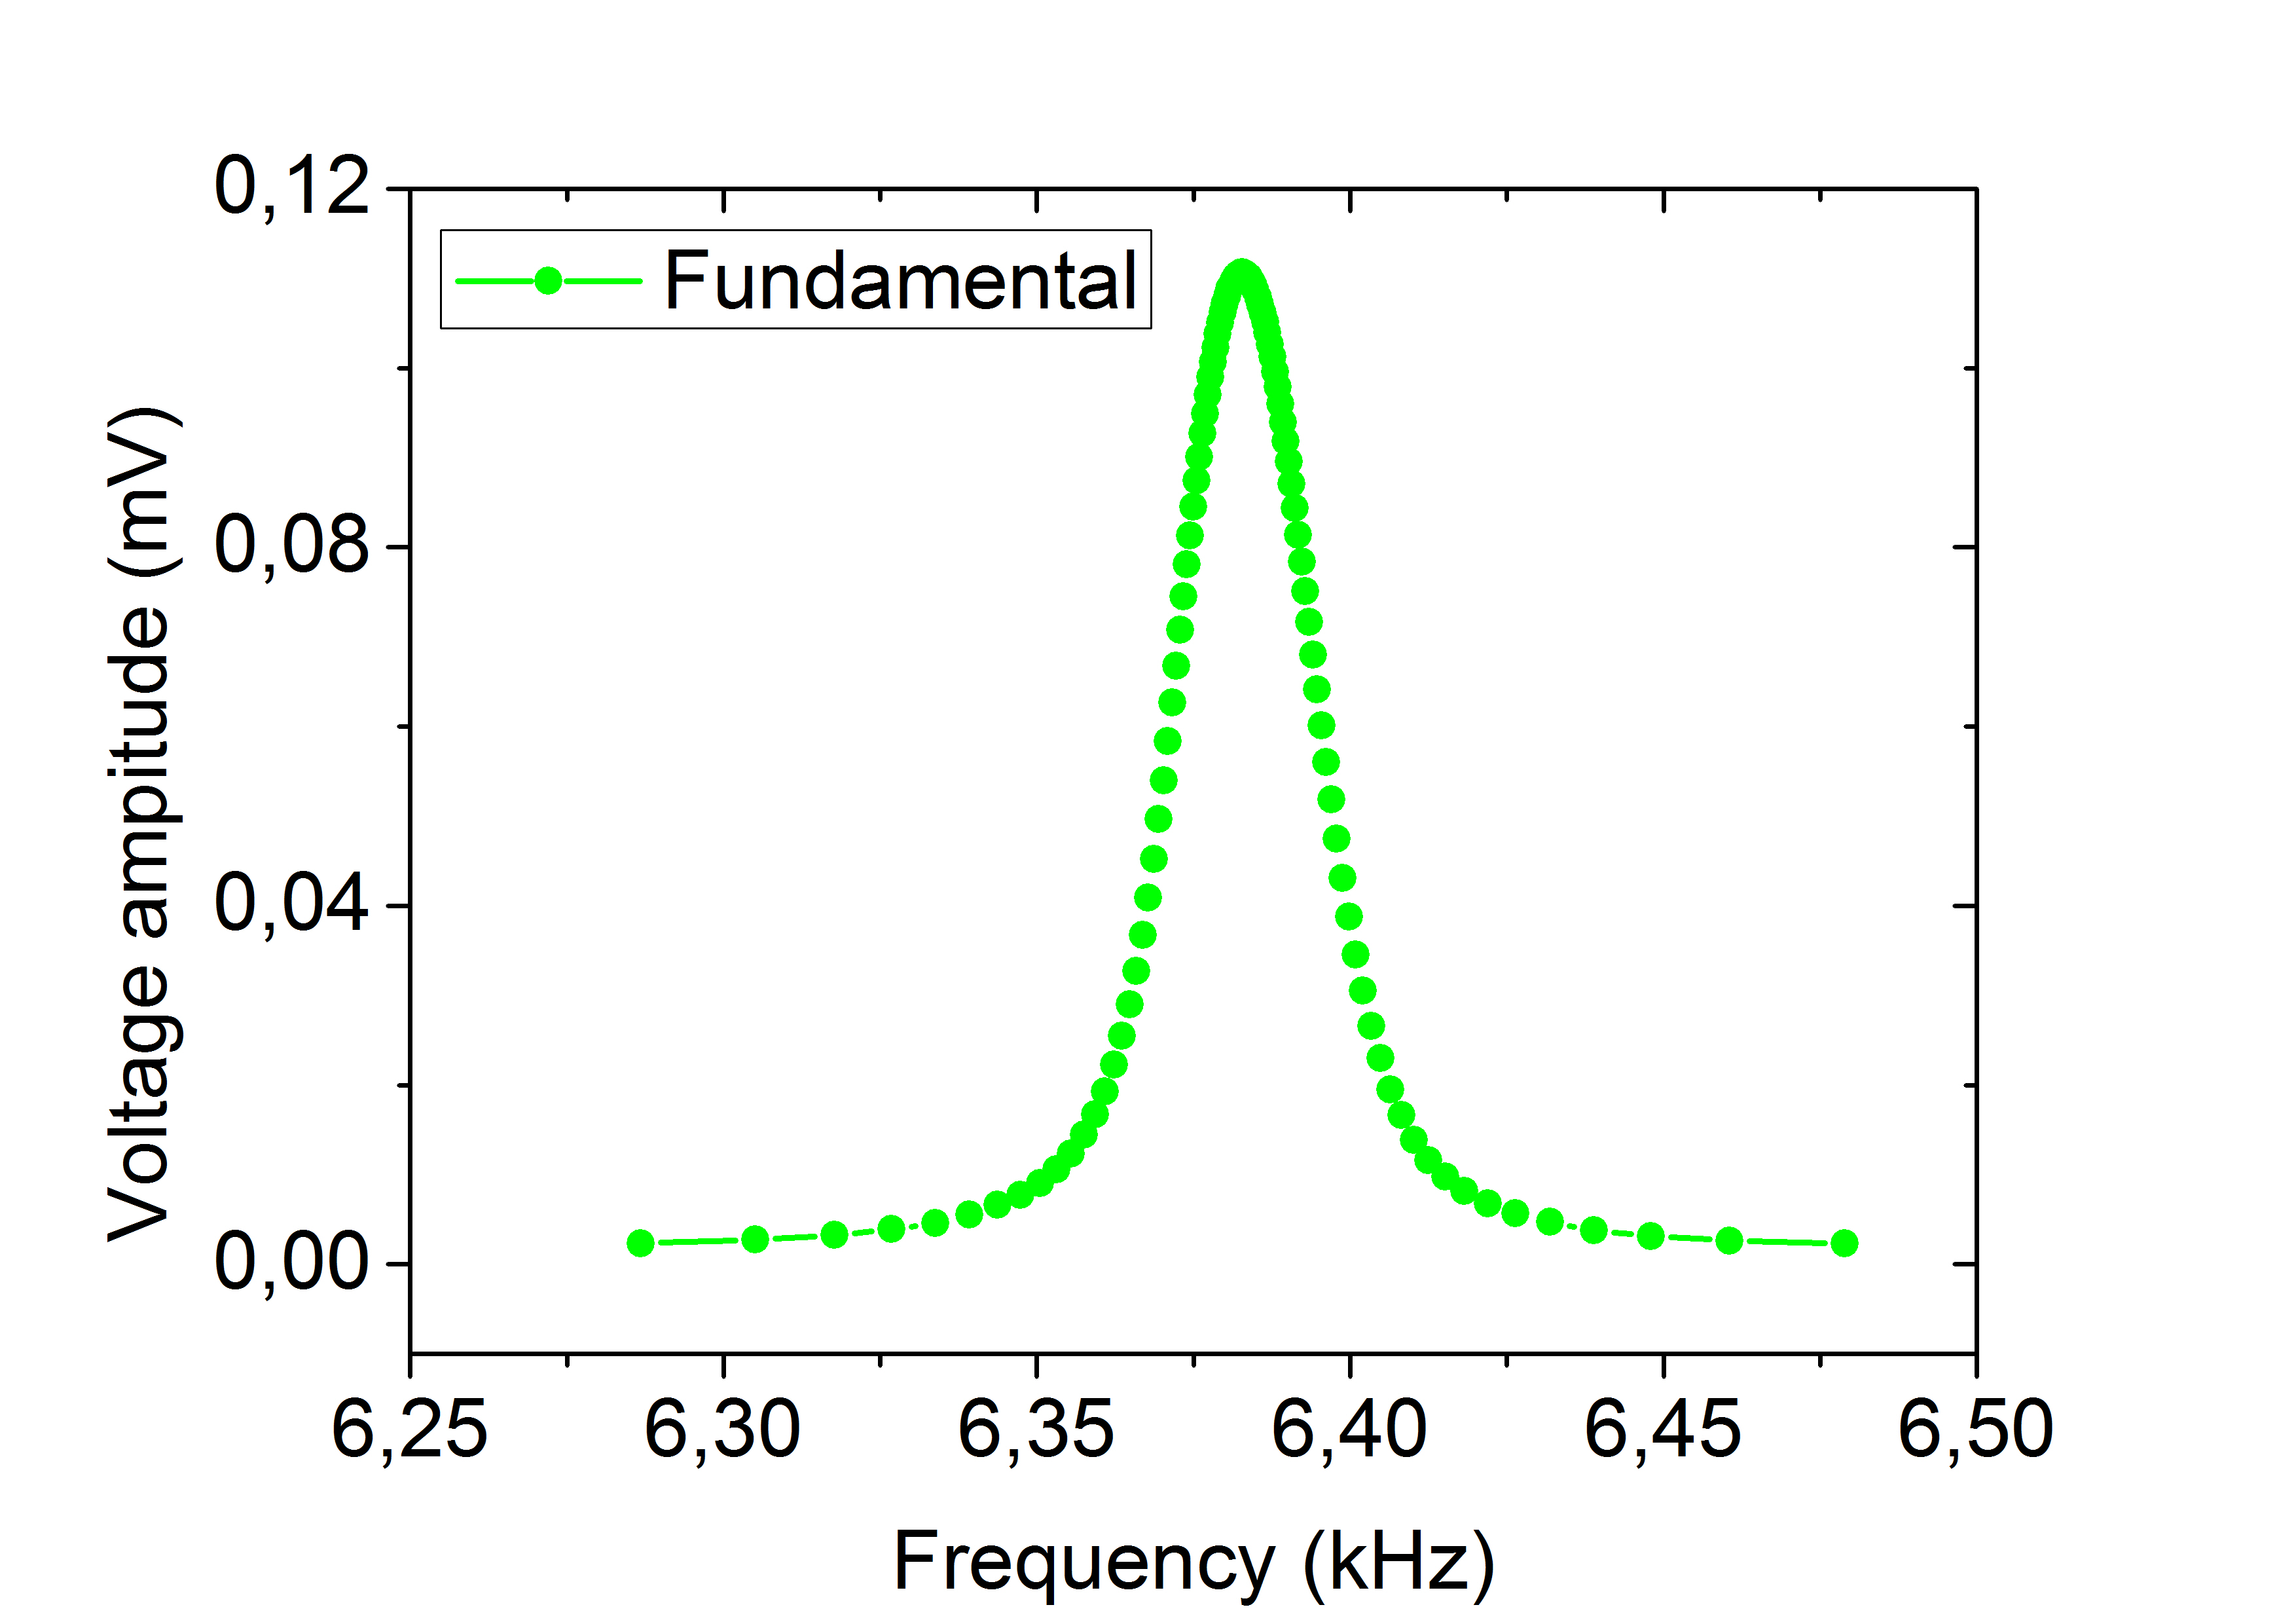
\includegraphics[width=0.49\textwidth]{graphs/TF_fund}
	\hfill
	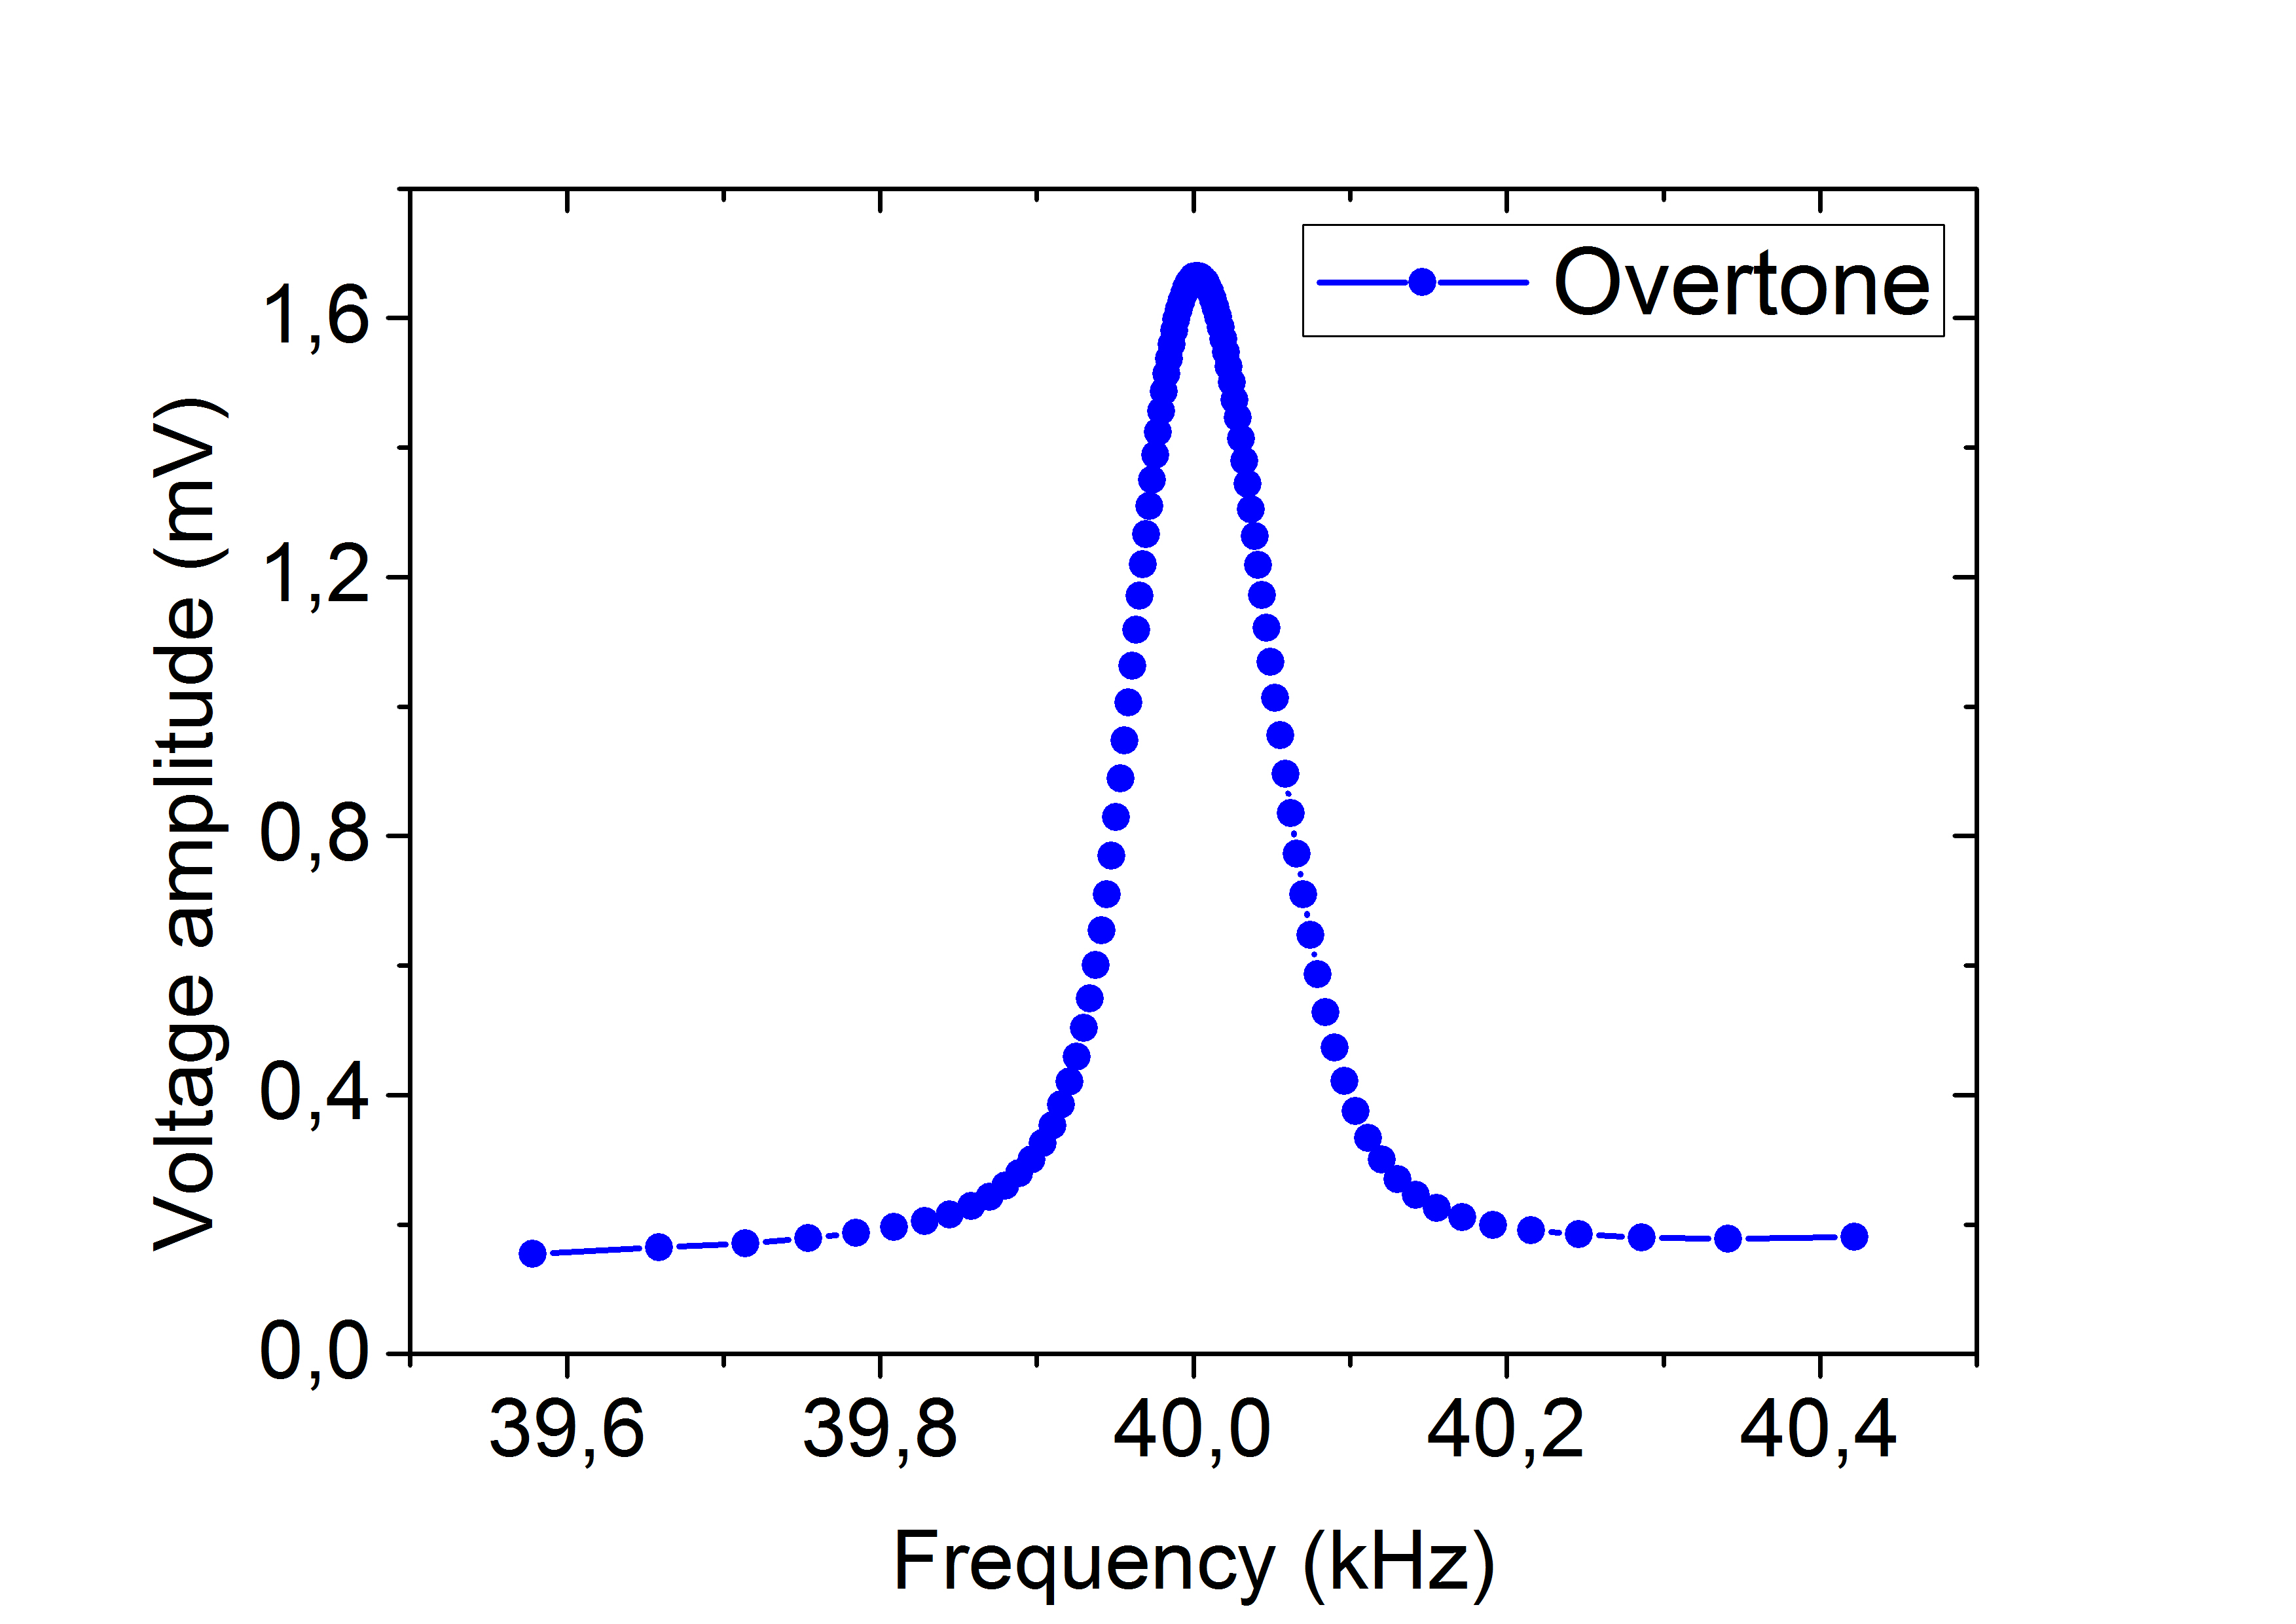
\includegraphics[width=0.49\textwidth]{graphs/TF_over}
	\caption{Left to right: Fundamental and overtone frequency sweeps.}
\end{figure}

The fitted full lines are Lorentzian curves with the general formula from \cite{forks}:

\begin{equation}
U(f) = U_{\text{off}} + U_0 \frac{(\Delta \omega)^2 \omega^2}{(\omega^2-\omega_0^2)^2 + (\Delta \omega)^2 \omega^2}\,.
\end{equation}

During this measurement the time step was set to 100ms and adaptive sampling was used due to the fact that we are more interested in the data-points sitting on the curve than outside. These frequency sweeps have been measured every time we changed the temperature or driving voltage because of possible resonant frequency shifts.

\subsection*{Frequency Mode for Second Sound}

The distance between the speaker and receiver is $ H= 54\unit{mm}$ and the second sound velocity is approximately $ u_2\approx20 \unit{m/s} $ within the range of temperatures $ (1.35\unit{K}-1.95\unit{K}) $. Using Eq.~(\ref{SSresonance}) we can estimate the second sound $ 1^{\ind{st}} $ resonant mode as $ f=u_2/2H \approx 185\unit{Hz} $.

\begin{figure}[h]
	\centering
	\vspace{-0.5cm}
	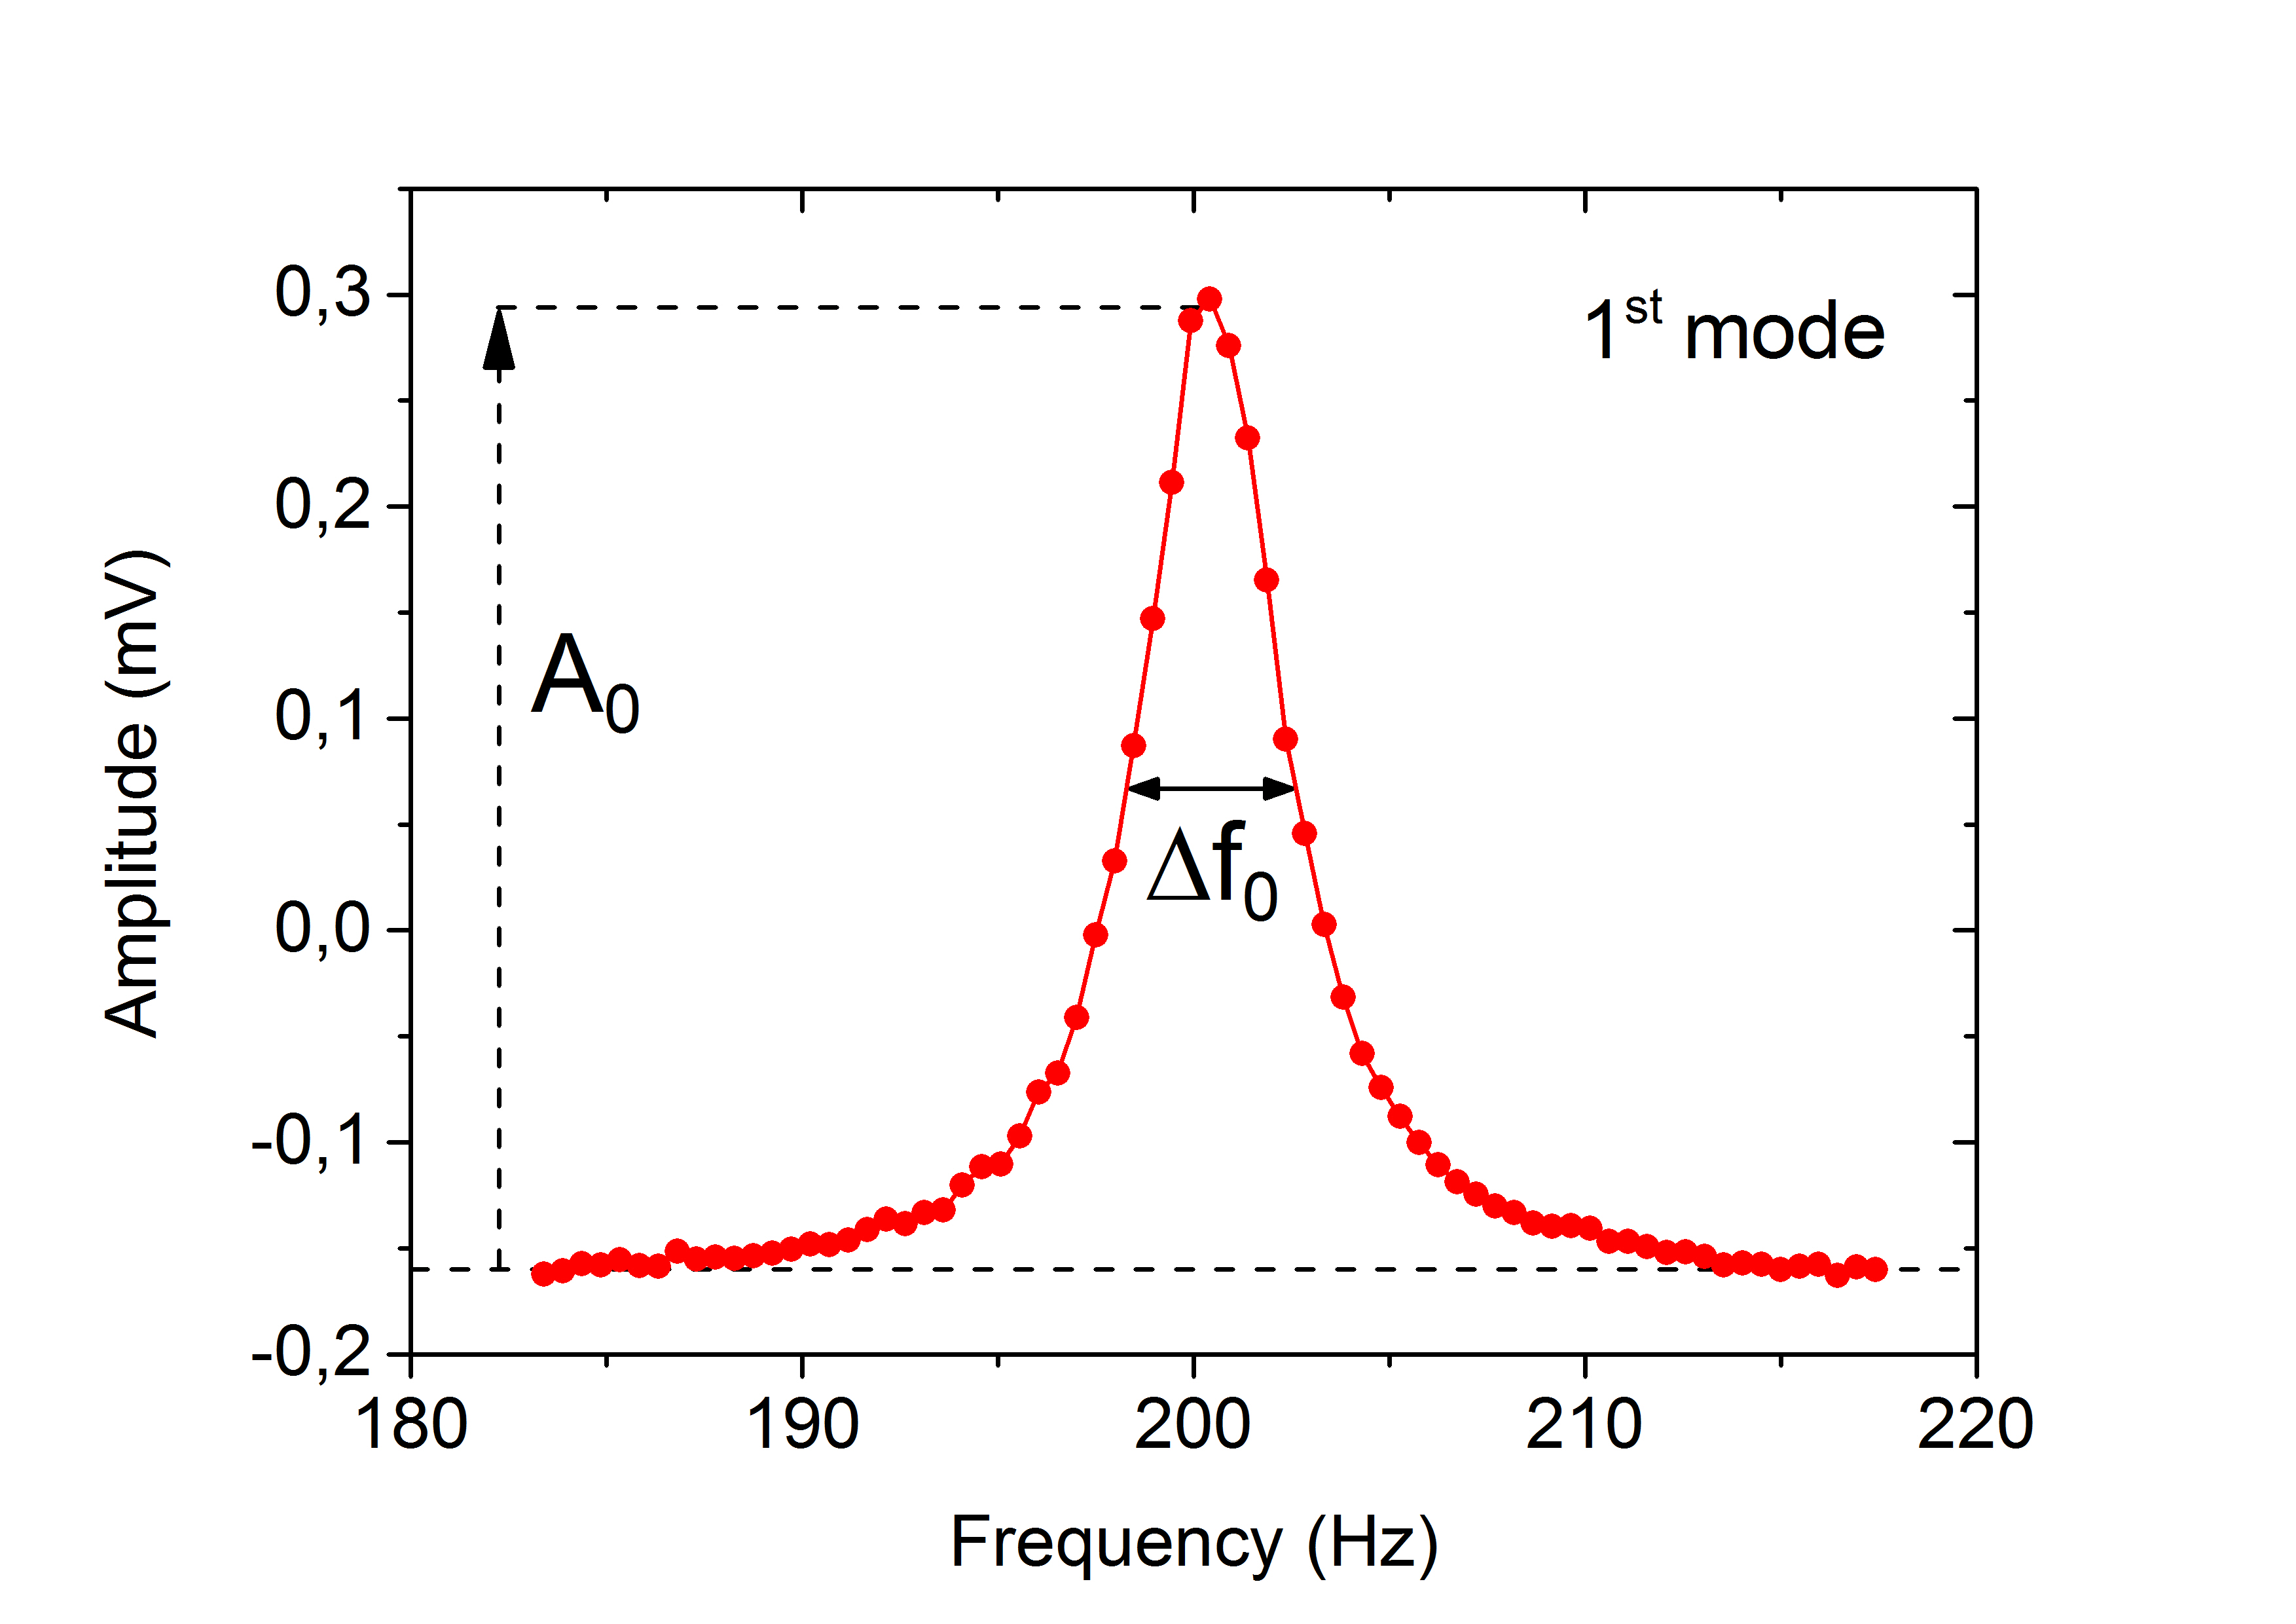
\includegraphics[width=0.6\textwidth]{graphs/SS_peak}
	\caption{$ 1^{\ind{st}} $ harmonic mode of second sound. Peak height $ A_0 $ and width $ \Delta f_0 $ are important parameters when inferring the vortex line density.}
\end{figure}

The observed $ 1^{\ind{st}} $resonance mode frequency slightly differs from the estimated one, due to finite lateral dimensions and non-ideal geometry.  Additionally, this mode is most sensitive in the middle of resonator, where the fork is located. Therefore, all the measurements including second sound were made at the $ 1^{\ind{st}} $ mode.

\subsection*{Constant Drive of Tuning Fork and Second Sound}

In this mode, the second sound ran continuously on its $ 1^{\ind{st}} $resonance mode whilst the fork oscillated also at its resonance (fundamental or overtone).

\begin{figure}[h]
	\centering
	\vspace{-0.5cm}
	\includegraphics[width=0.68\textwidth]{graphs/example}
	\caption{An example of suppressed second sound signal when the fork starts to oscillate. Time on the x-axis is measured since the execution of the measurement software. $ A_0-A$ corresponds to the signal drop, related to the equation of quantum turbulence \ref{L}.}
\end{figure}